%%%%%%%%% begin snippet
%% You need to add the package "tabularx".
%% Place the snippet right after \begin{document}

% need tabularx
\documentclass{article}
\usepackage{tabularx}
\usepackage{graphicx}
\usepackage{pdfpages}
\usepackage{listings}
\usepackage{subcaption}
\usepackage{verbatim}

\begin{document}
    \begin{titlepage}
           \begin{center}
                 \begin{huge}
                       %% Update assignment number here
                       \textbf{Assignment 3}
                 \end{huge}
           \end{center}

           \begin{center}
                 \begin{large}
                       Machine Learning 1, SS23
                 \end{large}
           \end{center}

           \begin{center}
                \begin{tabularx}{\textwidth}{|>{\hsize=.33\hsize}X|>{\hsize=.33\hsize}X|>{\hsize=.33\hsize}X|}

                       \hline
                       \multicolumn{3}{|c|}{\textbf{Team Members}} \\
                       \hline
                       Last name & First name & Matriculation Number \\
                       \hline
                       Grassl & Ifeoma & 12011965 \\
                       \hline
                       Royer & Christoph & 12004184 \\
                       \hline

                \end{tabularx}
           \end{center}

    \end{titlepage}

    \section{k-Nearest Neighbors}
    \subsection{Implementation}
    \textit{For implementation see} \texttt{task1\_1.py}

    \subsection{Application}
    Output for dataset 1:
    \begin{verbatim}
Test Score: 1.0
Dataset 1: {'k': 1}
    \end{verbatim}
    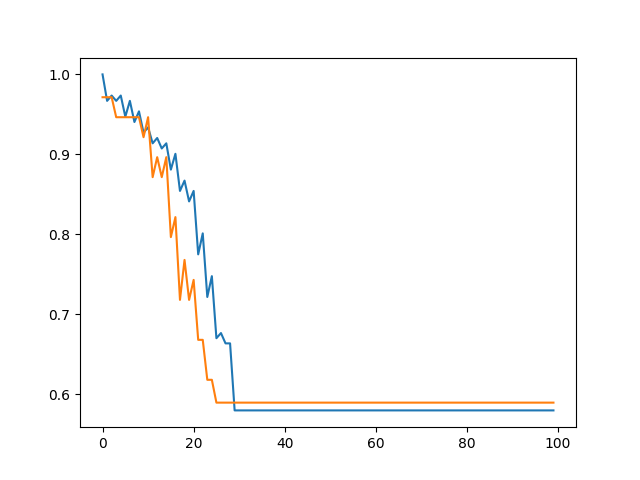
\includegraphics[width=\textwidth / 2]{plots/kmeans_loss_1}
    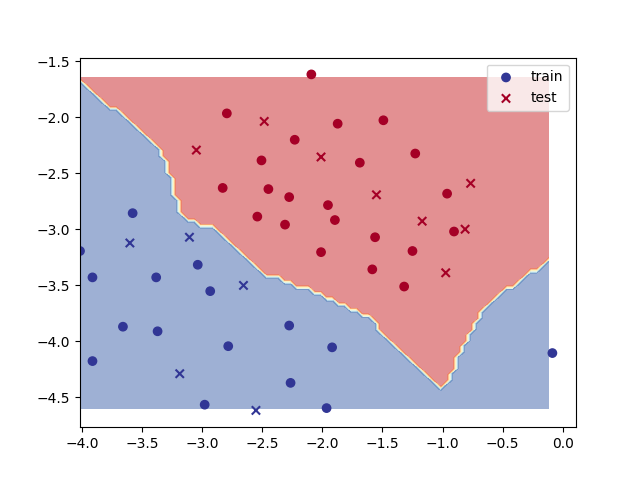
\includegraphics[width=\textwidth / 2]{plots/kmeans_boundary_1}

    Output for dataset 2:
    \begin{verbatim}
Test Score: 0.9953703703703703
Dataset 2: {'k': 1}
    \end{verbatim}
    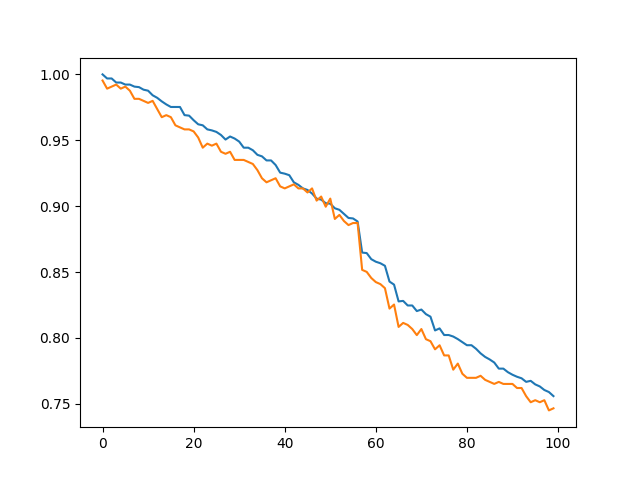
\includegraphics[width=\textwidth / 2]{plots/kmeans_loss_2}
    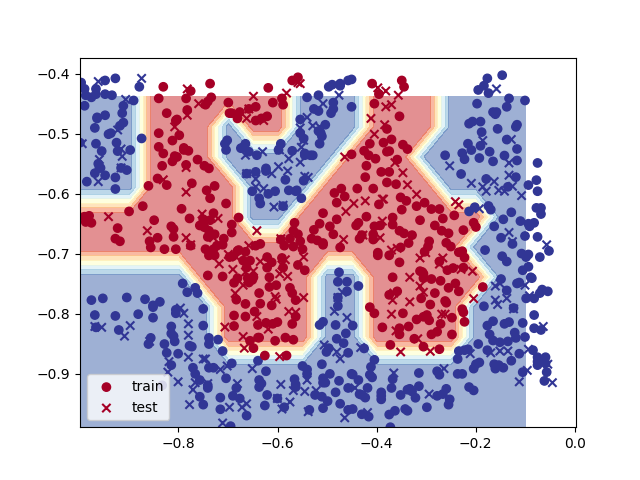
\includegraphics[width=\textwidth / 2]{plots/kmeans_boundary_2}

    Output for dataset 3:
    \begin{verbatim}
Test Score: 0.8867924528301887
Dataset 3: {'k': 3}
    \end{verbatim}
    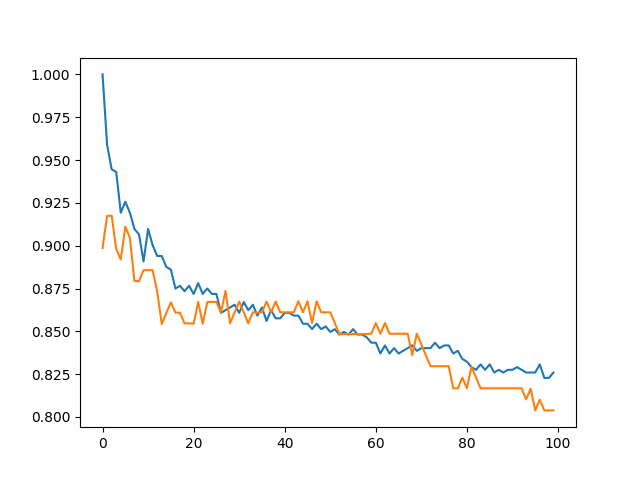
\includegraphics[width=\textwidth / 2]{plots/kmeans_loss_3}
    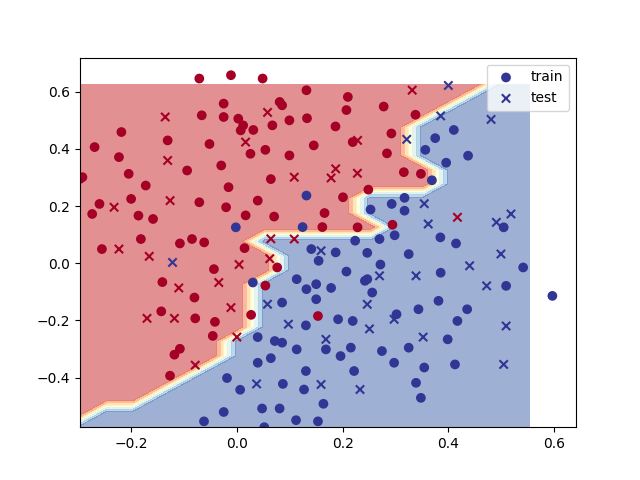
\includegraphics[width=\textwidth / 2]{plots/kmeans_boundary_3}

    \subsection{Choice of k}
    When $k=1$, the training accuracy is always $100\%$,
    since every point is its own nearest neighbor.
    This will often not generalize well though, as it takes every noisy sample as a new area for the given class.
    A high k on the other hand will be very robust against noise, but will have problems with complex decision boundaries,
    especially when there are relatively few training samples present near a complex boundary.

    \begin{verbatim}
Test Score for k=1: 0.7407407407407407
Cross-validated score for k=1: 0.7264162194394752
Test Score for k=5: 0.8009259259259259
Cross-validated score for k=5: 0.7666070363744782
Test Score for k=20: 0.7870370370370371
Cross-validated score for k=20: 0.7696362552176506
Test Score for k=50: 0.7824074074074074
Cross-validated score for k=50: 0.7557185450208707
Test Score for k=100: 0.7546296296296297
Cross-validated score for k=100: 0.6908288610614192

Best k: 15
Score: 0.7916666666666666
    \end{verbatim}

    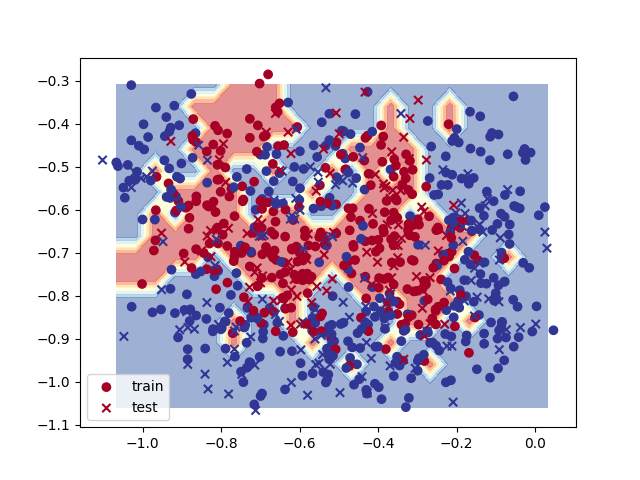
\includegraphics[width=\textwidth / 2]{plots/kmeans_noisy_boundary_1}
    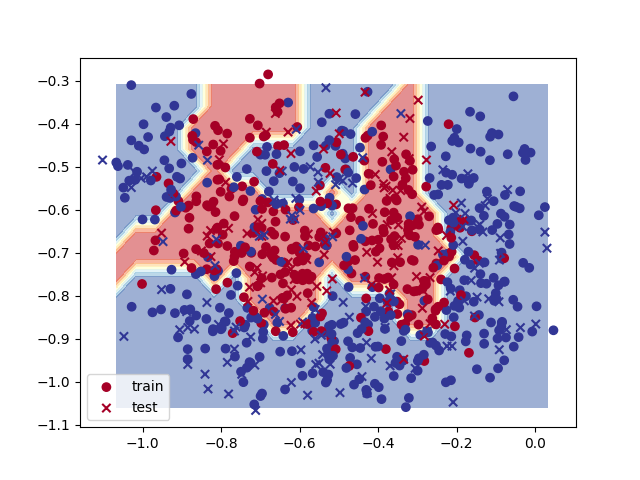
\includegraphics[width=\textwidth / 2]{plots/kmeans_noisy_boundary_5}
    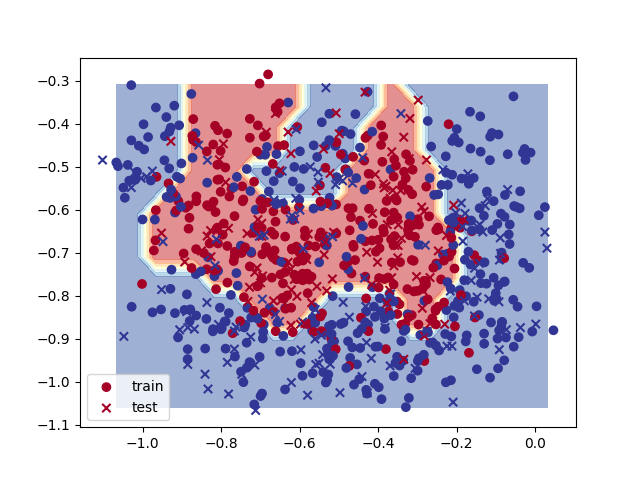
\includegraphics[width=\textwidth / 2]{plots/kmeans_noisy_boundary_20}
    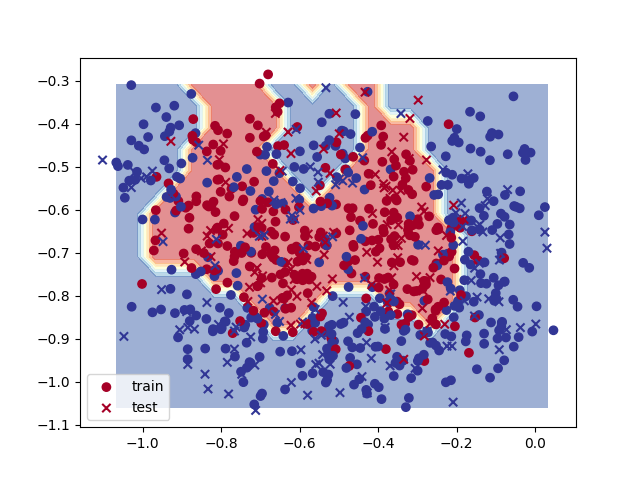
\includegraphics[width=\textwidth / 2]{plots/kmeans_noisy_boundary_50}
    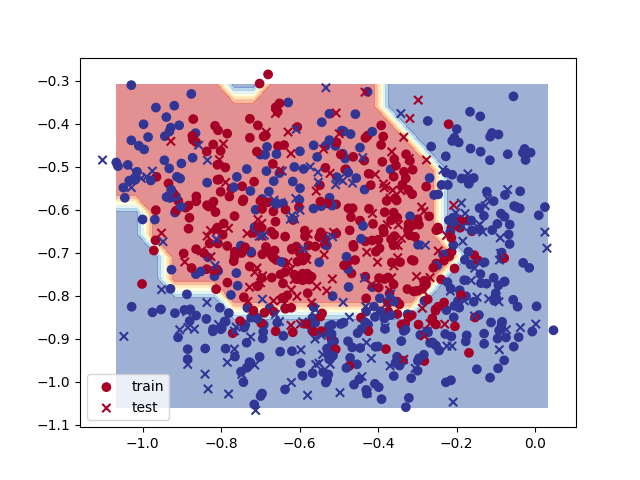
\includegraphics[width=\textwidth / 2]{plots/kmeans_noisy_boundary_100}
    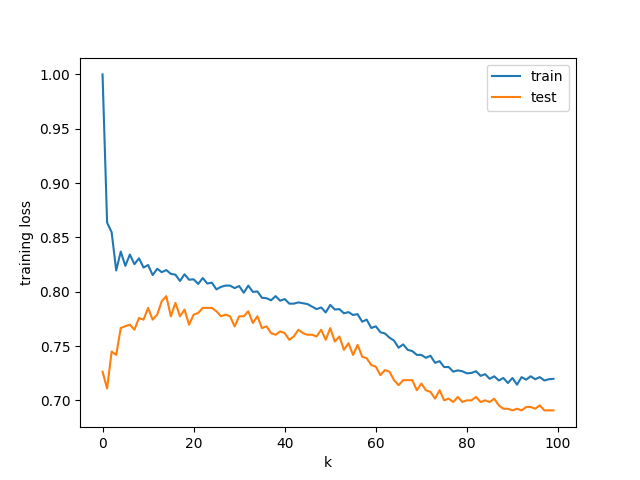
\includegraphics[width=\textwidth / 2]{plots/kmeans_noisy_loss}

    \section{Decision Trees \& Ensemble Methods}
    \subsection{Varying \texttt{max\_depth}}
    \begin{verbatim}
n_estimators = 1
Dataset 1: {'max_depth': 6}
Test Score: 0.8461538461538461
Dataset 2: {'max_depth': 19}
Test Score: 0.9444444444444444
Dataset 3: {'max_depth': 9}
Test Score: 0.8679245283018868
    \end{verbatim}
    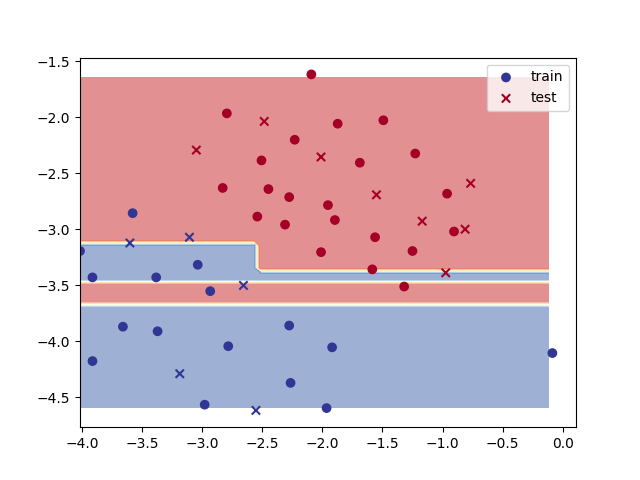
\includegraphics[width=\textwidth / 2]{plots/randomtree_nest1_1}
    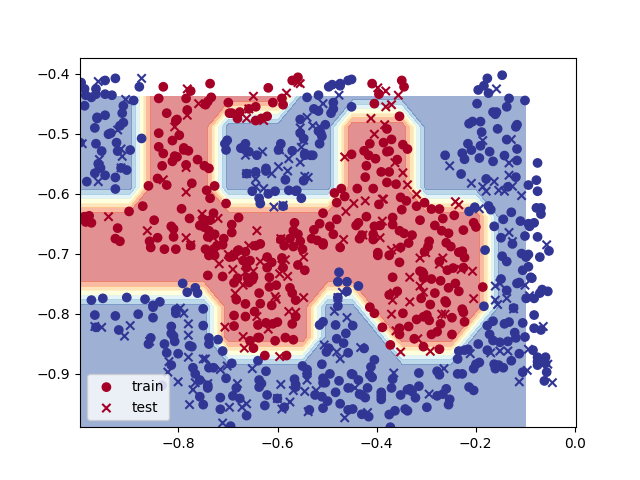
\includegraphics[width=\textwidth / 2]{plots/randomtree_nest1_2}
    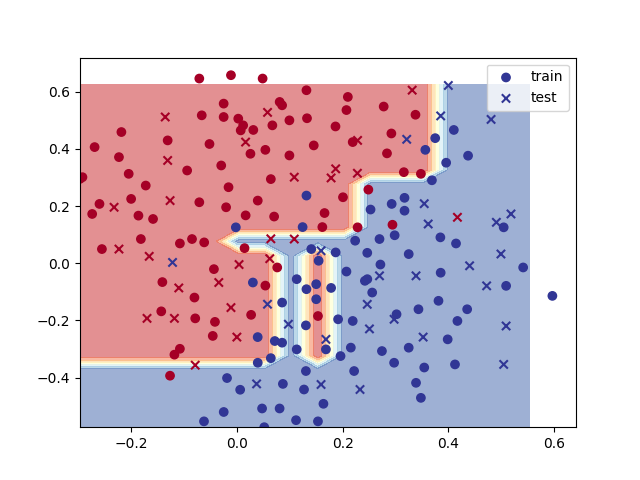
\includegraphics[width=\textwidth / 2]{plots/randomtree_nest1_3}

    \begin{verbatim}
n_estimators = 100
Dataset 1: {'max_depth': 5}
Test Score: 0.8461538461538461
Dataset 2: {'max_depth': 10}
Test Score: 0.9861111111111112
Dataset 3: {'max_depth': 18}
Test Score: 0.8867924528301887
    \end{verbatim}
    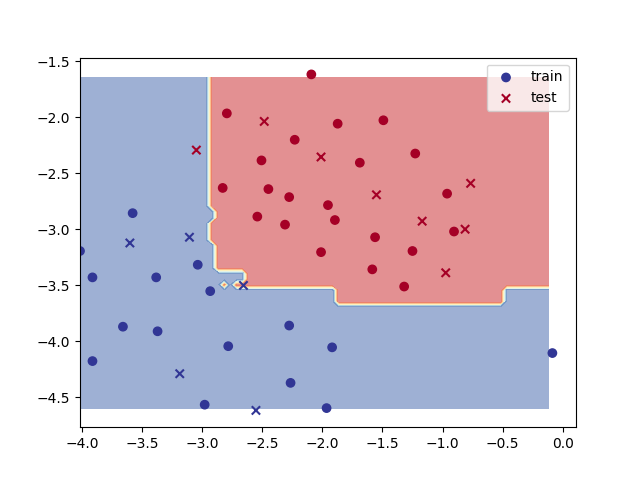
\includegraphics[width=\textwidth / 2]{plots/randomtree_nest100_1}
    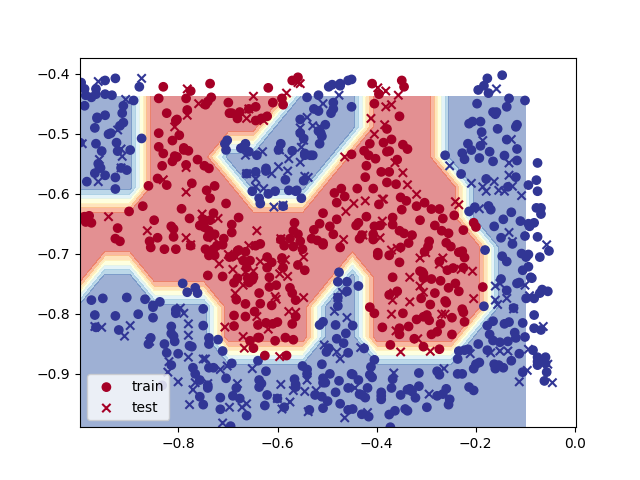
\includegraphics[width=\textwidth / 2]{plots/randomtree_nest100_2}
    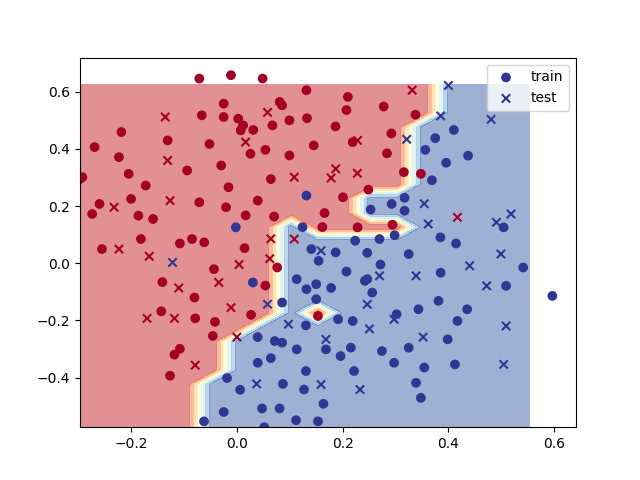
\includegraphics[width=\textwidth / 2]{plots/randomtree_nest100_3}

    The classifier is less affected by outliers as the number of trees increases.
    This is because many of the trees (mis)interpret the outliers differently, and thus the error averages out with an
    averaged classification over all trees.


    \subsection{RFECV}
    The following bar chart shows the most important features in the data set.
    We can plainly see for example, that feature number 13 is the most important.
    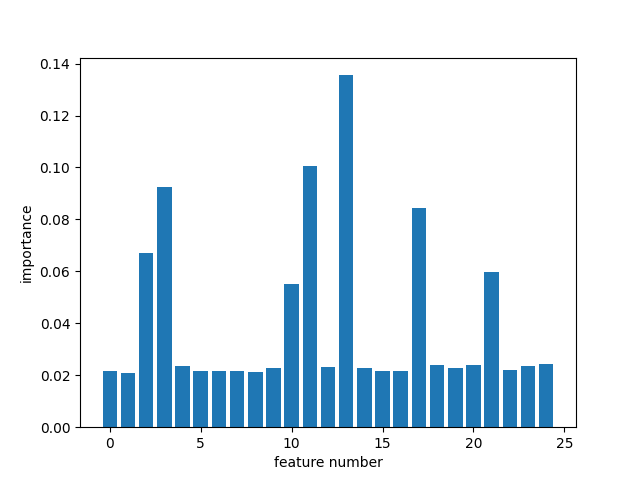
\includegraphics[width=\textwidth]{plots/randomtree_feat_importances}
    The following is the output of the unpruned part of the script:
    \begin{verbatim}
Score of Random Forest: 0.684
Score of SVC: 0.708
    \end{verbatim}

    The following is the output of the pruned part of the script:
    \begin{verbatim}
Score of SVC on pruned data: 0.744
    \end{verbatim}
    We can see that we got a better score on the test data compared to taking all of the features.
    This tells us that many of the features in the dataset were redundant or irrelevent to the classification,
    which is why the classifier performed better without considering them.
\end{document}

%%%%%%%%% end snippet
